\documentclass[a4paper,12pt]{book}
\usepackage{mathptmx}
\usepackage{hyperref}
\usepackage{cancel}
\usepackage{amsmath}
\usepackage{amssymb}
\usepackage{graphicx}
\author{Gábor Hadházy and Tamás Hadházy}
\title{Mathematics}
\date{\today}

\begin{document}
\maketitle

\tableofcontents

% Chapter 1 - Algebra
\chapter{Algebra and Pre-calculus}
The first chapter is about algebra. It will cover the topics that was written by Gábor Hadházy and Tamás Hadházy. Algebra and Pre-calculus are the foundation of mathematics. It is important to understand the concepts of algebra and pre-calculus before moving on to more advanced topics.

\section{Essentials}
This section will cover the essentials in order to get started. 
\subsection{The set of Real numbers}
\begin{itemize}
    \item $\mathbb{N} = \{1, 2, 3, ...\}$ - - The set of natural numbers. 
    \item $\mathbb{Z} = \{..., -2, -1, 0, 1, 2, ...\}$ - The set of integers.
    \item $\mathbb{Q} = \{\frac{a}{b} | a, b \in \mathbb{Z}, b \neq 0\}$ - The set of rational numbers. 
    \item $\mathbb{I}$ - The set of Irrational Numbers(Real numbers that are not rational). 
    \item $\mathbb{R} = \mathbb{Q} \cup \mathbb{I}$
\end{itemize}


\subsection{The properties of Real numbers}
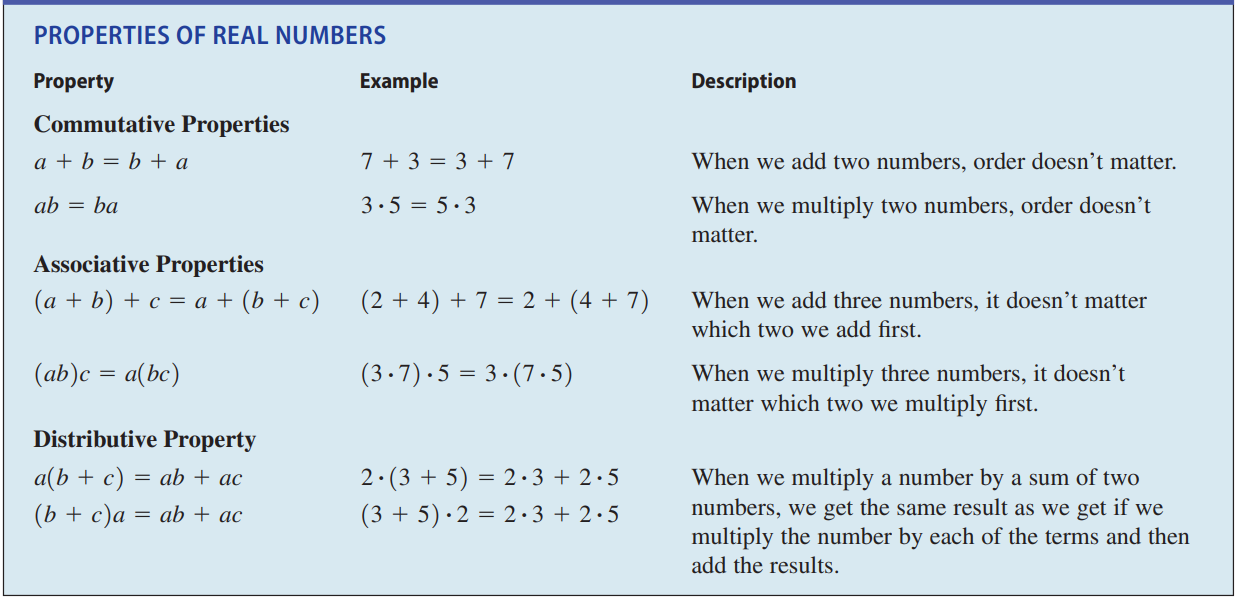
\includegraphics[width=1.1\textwidth]{algebra-pre-calculus/essentials/properties.png}

\subsection{Addition and Subtraction}
The number 0 is special for addition; it is called the additive identity because $a+0=a$ for any real number $a$. Every real number $a$ has a negative, $-a$, that satisfies $a+(-a)=0$. Subtraction is the operation that undoes addition; to subtract a number from another, we simply add the negative of that number. By definition
$$
a-b=a+(-b)
$$
To combine real numbers involving negatives, we use the following properties.
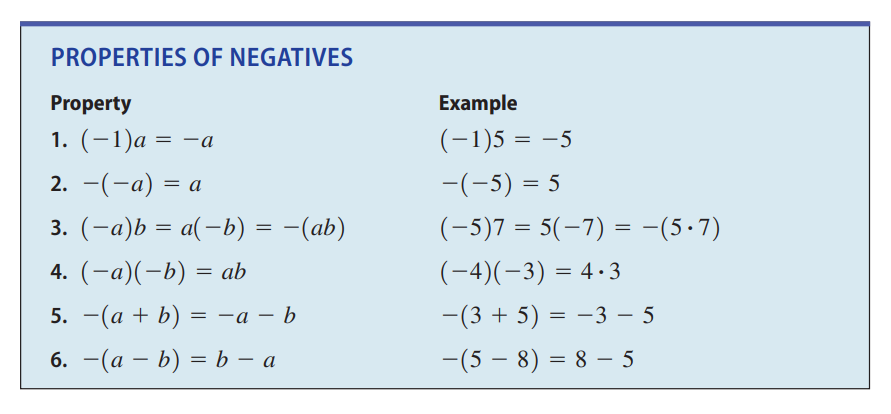
\includegraphics[width=1.1\textwidth]{algebra-pre-calculus/essentials/properties_addition_subtraction.png}

Property 6 states the intuitive fact that $a-b$ and $b-a$ are negatives of each other. \\
Property 5 is often used with more than two terms:
$$
    -(a+b+c)=-a-b-c
$$

\subsection{Multiplication and Division}
The number 1 is special for multiplication; it is called the \textbf{multiplicative identity} because $a \cdot 1=a$ for any real number $a$. Every nonzero real number $a$ has an inverse, $1 / a$, that satisfies $a \cdot(1 / a)=1$. Division is the operation that undoes multiplication; to divide by a number, we multiply by the inverse of that number. If $b \neq 0$, then, by definition,
$$
a \div b=a \cdot \frac{1}{b}
$$
We write $a \cdot(1 / b)$ as simply $a / b$. We refer to $a / b$ as the quotient of $a$ and $b$ or as the fraction $a$ over $b$; $a$ is the numerator and $b$ is the denominator (or divisor). To combine real numbers using the operation of division, we use the following properties. \\
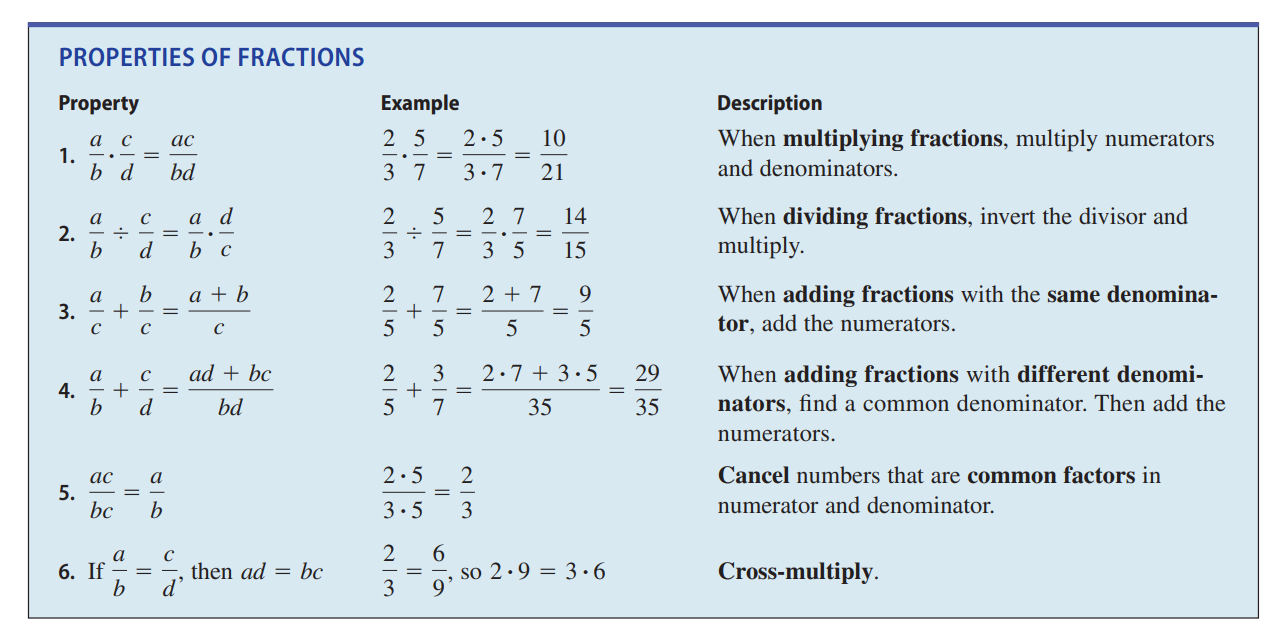
\includegraphics[width=1.1\textwidth]{algebra-pre-calculus/essentials/properties_multiplication_division.png}

When adding fractions with different denominators, we don’t usually use Property 4.
Instead we rewrite the fractions so that they have the smallest possible common denominator (often smaller than the product of the denominators), and then we use Property 3. This
denominator is the Least Common Denominator (LCD) described in the next example.

\subsection{Using the LCD to Add Fractions}

Evaluate: $\frac{5}{36}+\frac{7}{120}$
\textbf{Solution.} Factoring each denominator into prime factors gives
$$
36=2^2 \cdot 3^2 \quad \text { and } \quad 120=2^3 \cdot 3 \cdot 5
$$
We find the least common denominator (LCD) by forming the product of all the prime factors that occur in these factorizations, using the highest power of each prime factor. Thus the LCD is $2^3 \cdot 3^2 \cdot 5=360$. So
$$
\begin{aligned}
\frac{5}{36}+\frac{7}{120} & =\frac{5 \cdot 10}{36 \cdot 10}+\frac{7 \cdot 3}{120 \cdot 3} & \text { Use common denominator } \\
& =\frac{50}{360}+\frac{21}{360}=\frac{71}{360} & \begin{array}{l}
\text { Property } 3: \text { Adding fractions with the } \\
\text { same denominator }
\end{array}
\end{aligned}
$$

\subsection{Real line}

The real numbers can be represented by points on a line, as shown below. The
positive direction (toward the right) is indicated by an arrow. We choose an arbitrary
reference point O, called the origin, which corresponds to the real number 0. Given any
convenient unit of measurement, each positive number x is represented by the point on
the line a distance of x units to the right of the origin, and each negative number -x is
represented by the point x units to the left of the origin. The number associated with the
point P is called the coordinate of P, and the line is then called a coordinate line, or a
real number line, or simply a real line. Often we identify the point with its coordinate
and think of a number as being a point on the real line.

\begin{align*}
    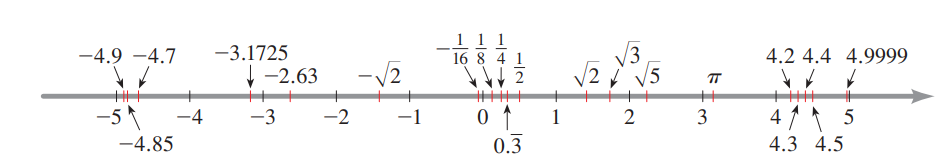
\includegraphics[width=1.1\textwidth]{algebra-pre-calculus/essentials/real-line.png}
\end{align*}

\section{Absolute Value and Distance}
The absolute value of a number $a$, denoted by $|a|$ , is the distance from $a$ to 0 on
the number line. Distance is always positive or zero, so we have
$|a|\geq0$ for every number $a$. Remembering that $-a$ is positive when $a$ is negative, we have the following definition.

\begin{equation*}
    |a| = \begin{cases}
        \;a  & \textnormal{if} \ a \geq 0 \\
        \;-a & \textnormal{if} \ a < 0
    \end{cases}
\end{equation*}

(a) $|3|=3$ \\
(b) $|-3|=-(-3)=3$ \\
(c) $|0|=0$ \\
(d) $|3-\pi|=-(3-\pi)=\pi-3 \quad($ since $3<\pi \quad \Rightarrow \quad 3-\pi<0)$

\subsection{Properties of Absolute Value}
\begin{enumerate}
    \item $|a| \geq 0$
    \item $|a|=|-a|$
    \item $|a b|=|a||b|$
    \item $\displaystyle \left|\frac{a}{b}\right|=\frac{|a|}{|b|}$
    \item $|a+b| \leq|a|+|b|$
\end{enumerate}

\subsection{Distance Between Points on the Real line}

What is the distance on the real line between the numbers -2 and 11? From
Figure 11 we see that the distance is 13. We arrive at this by finding either
$ |11-(-2)|=13$ or $|(-2)-11=13|$. From this observation we make the following definition. \\

If $a$ and $b$ are real numbers, then the \textbf{distance} between the points $a$ and $b$ on the real line is: \\
$$ d(a,b)=|a-b| $$

From the Property 6 of negatives it follows that
$$ |b-a| = |a-b|$$
$$ |3-7| = |7-3| = 4 $$

This confirms that, as we would expect, the distance from a to b is the same as the
distance from b to a.

\textbf{Example.} The distance between then numbers -8 and 2 is $d(-8,2)=|-8-2|=|-10|=10$.

\subsubsection*{Exercises}
For Exercises please download the book from here(\url{https://faculty.ksu.edu.sa/sites/default/files/precalculus-mathematics_for_calculus-j._stewart_l._redlin_and_s._watson-cengage_learning_7th_edition_2015.pdf}) and you can go to the 37th page for exercises.  % Section 1 - Essentials
\section{Exponentiation}
When starting out with Exponentiation it is important first to understand the different parts of an exponential expression, so let's consider:
$$b^x = \underbrace{b \cdot b \cdot ... \cdot b}_{x \ times}$$
\begin{itemize}
  \item $b$ is the \textbf{base}.
  \item $x$ is the \textbf{exponent}.
\end{itemize}

As a reminder $ x^0 = 1 $

Let's discuss the different rules of Exponentiation:
\subsection{Product Rule}
To find the product of two exponential expression with the same base, add the exponents. 
$$ x^{n} \cdot x^{m} = x^{n+m} $$

\subsection{Quotient Rule}
When two exponential expressions with the same base are divided,  to find their quotient subtract their exponents. 
$$ \frac{x^n}{x^m} = x^{n-m} $$

\subsection{Power Rule}
When you raise an power to a power in an exponential expression to get the product, multiply the exponents
$$ (x^{n})^{m} = x^{n \cdot m} $$ 
$$ OR $$
$$ (x^{n})^{m} = \underbrace{x^n \cdot ... \cdot x^n}_{m \ times} $$
Here it is proven that the power rule is simply just the product rule.

\subsection{Negative Exponents}
When dealing with negative exponents this equation will apply: 
$$ x^{-n} = \frac{1}{x^n} $$

Since, 
$$ \frac{1}{x} = \frac{x^0}{x^1} = x^{0-1} = x^{-1} $$
It is important to note that this is just only one way of proving this, there are a couple more. 

\subsection{Fractional Exponents}
$$ \large x^{\frac{1}{n}} = \sqrt[n]{x} $$
The proof of this can be found in the next section \hyperref[sec:radicals]{Radicals(click to redirect)}.

\subsection{Additional rules}
Distribute an exponent over a product: $(x \ y)^{n} = x^{n} \ y^{n}$ \\
Distribute an exponent over a quotient: $  (\frac{a}{b})^{n} = \frac{a^{n}}{b^{n}}$

\begin{align*}
  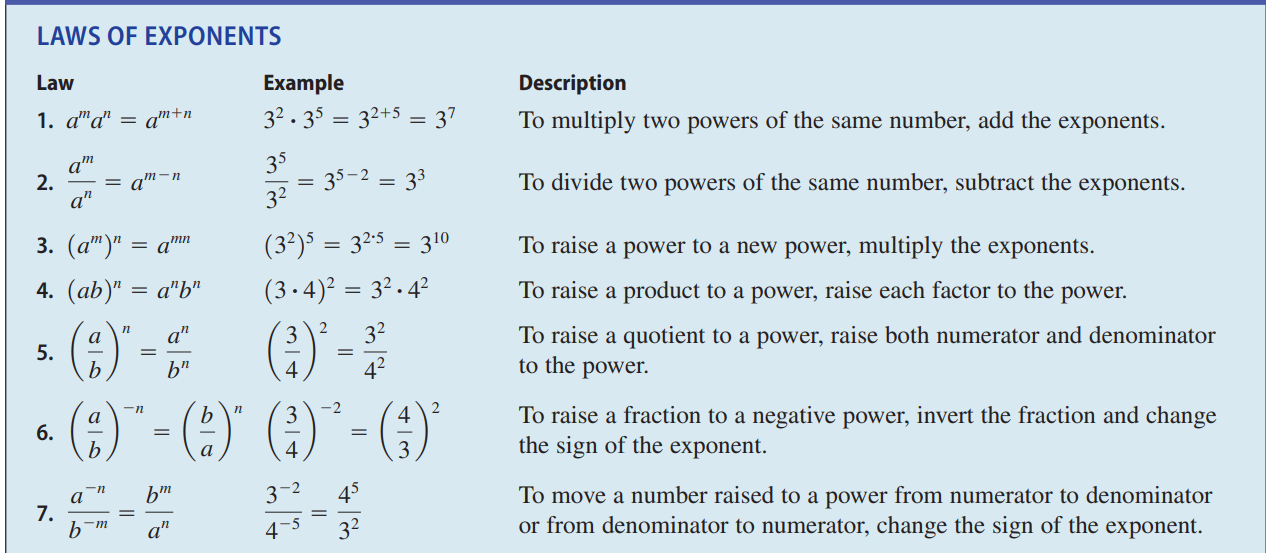
\includegraphics[width=1.2\textwidth]{algebra-pre-calculus/exponentiation/laws-of-exponents.png}
\end{align*}

\newpage % Section 2 - Exponentiation
\label{sec:radicals}
\section{Radicals}
$$ \large \sqrt[n]{x} $$
\begin{itemize}
  \item $x$ is the \textbf{radicand}.
  \item $n$ is the \textbf{index}(nth root).
  \item $\large \sqrt[n]{x}$ expression is the \textbf{radical}
\end{itemize}

As promised let's look at the fractional exponent equation. If $n$ is a positive integer that is greater than $1$ and a is a real number then,
$$ \sqrt[n]{a} = a^{\frac{1}{n}} $$

We are often referring the left side of the equation as the \textbf{radical form} and the right side of the equation as the \textbf{exponent form}

\subsubsection{Proof}
In order to prove this equation we can establish first this: 
$$ (a^{\frac{1}{n}})^{n} = a^{n \cdot \frac{1}{n}} = a^{\frac{n}{n}} = a $$
Let's take an example to avoid confusion: 
$$ (9^{\frac{1}{2}})^2 = 9^{\frac{1}{2} \cdot2} = 9^{\frac{2}{2}} = 9 $$

To put this into words $ 9^{\frac{1}{2}} $ is the number that when squared will return back $ 9 $. In other words this is exactly what it meant by the root(in this case square root) which will return back the number that when squared it will be 9. Therefore: 
$$ 9^{\frac{1}{2}} =  \sqrt[2]{9} = 3 $$

Since,
$$ (3)^2 = 9 = (9^{\frac{1}{2}})^2 $$

Therefore the equation has been proven: 
$$ \sqrt[n]{a} = a^{\frac{1}{n}} $$

It is very important to note a misconception here. The index is required in these radical expressions to make sure that we correctly evaluate the radical. There is one exception to this rule and that is square root.
$$ \sqrt[2]{a} = \sqrt[]{a} $$
In every other cases we \textbf{must} define the index, because otherwise it will be considered as a square root, Whenever working with square roots the index can be omitted.

\subsubsection{General rational exponent}
Since, $ a^{\frac{1}{n}} = \sqrt[n]{a} $.
Let's establish the general rational exponent in terms of radicals as follows. 
$$ a^{\frac{m}{n}} = (a^{\frac{1}{n}}) ^{m} = (\sqrt[n]{a})^m $$
$$ OR $$
$$ a^{\frac{m}{n}} = (a^m) ^{\frac{1}{n}} = \sqrt[n]{a^m} $$

Since being aware of the \textbf{Associative Property of Multiplication}, the order of the multiplication can be changed. 

Therefore, 
$$ a^{\frac{m}{n}} = \sqrt[n]{a^m} $$

\subsection{Properties of radicals}
\begin{itemize}
  \item $\sqrt[n]{a^n} = a$ \ This is simply true because when trying to find the $n$th root of a number and  also raising the number to that power then that's simply will be equal to the number.  \\
Consider this as an example,
$$ \sqrt[]{9^2} = \sqrt[]{81} = 9$$
   \item $ \sqrt[n]{ab} = \sqrt[n]{a} \sqrt[n]{b} $ \\
   To prove this consider this, \\
    1. Start with the left-hand side (LHS) of the equation,
    $ \sqrt[n]{ab} $ Using the definition of the nth root:
    $ \sqrt[n]{ab} = (ab)^{\frac{1}{n}} $ \\
    2. Next apply the product rule of exponents, which states that $ a^m \cdot a^n = a^{m+n} $ Therefore, $ (ab)^{\frac{1}{n}} = a^{\frac{1}{n}} \cdot b^{\frac{1}{n}} $ \\ 
    3. Now, rewrite the exponents as radicals:
    $ a^{\frac{1}{n}} $ is equivalent to $ \sqrt[n]{a} $ and $ b^{\frac{1}{n}} $ is equivalent to $ \sqrt[n]{b} $ \\
    4. So, we have: $ a^{\frac{1}{n}} \cdot b^{\frac{1}{n}} = \sqrt[n]{a} \cdot \sqrt[n]{b} $ \\
    5. Finally this proves that: $ \sqrt[n]{ab} = \sqrt[n]{a} \cdot \sqrt[n]{b} $
    \item $ \large \sqrt[n]{\frac{a}{b}} = \frac{\sqrt[n]{a}}{\sqrt[n]{b}} $ To prove this consider this, \\
    1. As previously Start with the left-hand side (LHS) of the equation: $ \sqrt[n]{\frac{a}{b}} $ \\
    2. Now using the definition of the nth root: $ \sqrt[n]{\frac{a}{b}} = \left(\frac{a}{b}\right)^{\frac{1}{n}} $ \\
    3. Apply the power rule of the exponents which states that: \\ $ (a^m)^{\frac{1}{n}} = a^{m \cdot \frac{1}{n}} = a^{\frac{m}{n}}$, Therefore when we are dealing with a fraction as the base it is the same when dealing with numbers that are not fractions: 
$$ \left(\frac{a}{b}\right)^{\frac{1}{n}} = \frac{a^{\frac{1}{n}}}{b^{\frac{1}{n}}} $$ Since, \\
$$ (\frac{a}{b})^c = \frac{a^c}{b^c} $$ \\
With an example: $ (\frac{a}{b})^2 = \frac{a}{b} \cdot \frac{a}{b} = \frac{a^2}{b^2} $ \\
	4. Now rewrite the exponents as radicals: $ a^{\frac{1}{n}} $ is equivalent to $ \sqrt[n]{a} $ and  $b^{\frac{1}{n}}$ is equivalent to $ \sqrt[n]{b} $ \\
	5. So, we have: 
	$$ \frac{a^{\frac{1}{n}}}{b^{\frac{1}{n}}} = \frac{\sqrt[n]{a}}{\sqrt[n]{b}} $$ \\
	6. Finally, this proves that: 
	$$ \sqrt[n]{\frac{a}{b}} = \frac{\sqrt[n]{a}}{\sqrt[n]{b}} $$ \\
	\\
	
	\item Also note that while we can “break up” products and quotients under a radical we can’t do the same thing for sums or differences. In other words,
	$$ \sqrt[n]{a+b} \neq \sqrt[n]{a}+ \sqrt[n]{b}  $$ 
	$$ AND $$
	$$ \sqrt[n]{a-b} \neq \sqrt[n]{a}- \sqrt[n]{b} $$ \\
These can simply be proven by examples, 
$$ 5 = \sqrt25 = \sqrt{9+16} \neq \sqrt9 + \sqrt16 = 3+4 = 7 $$

\end{itemize} % Section 3 - Radicals
\section{Factorials}
In mathematics, the factorial of a non-negative integer(whole number (not a fractional number) that can be positive, negative, or zero.) $ n $, denoted by $ n! $, is the product of all positive integers less than or equal to $ n $ \\

$$ 5! = 5 \cdot 4 \cdot 3 \cdot 2 \cdot 1 = 123 $$ \\
Generically expressing, 
$$ n! = n \cdot (n-1) \cdot (n-2) \cdot (n-3) \cdot ... \cdot 3 \cdot 2 \cdot 1 $$

\subsection{Operations with factorials}
Let's clarify a couple of easy examples, 
$$ 2! + 3! = 2 \cdot 1 + 3 \cdot 2 \cdot 1 = 8 $$ 
$$ 3! 4! = 3 \cdot 2 \cdot 1 \cdot 4 \cdot 3 \cdot 2 \cdot 1 = 144 $$ \
When it comes to a fraction of factorials there are some tricks to implement: 
$$ \frac{9!}{7!} = \frac{9 \cdot 8 \cdot 7!}{7!} = 9 \cdot 8 = 72$$
Since, $ 7! = 7 \cdot 6 \cdot 5 \cdot 4 \cdot 3 \cdot 2\cdot 1 $ \\
Consider a similar example: 
$$ \frac{4!5!}{6!} = \frac{(4 \cdot 3 \cdot 2 \cdot 1)(5!)}{6 \cdot 5!} = \frac{24}{6} = 4 $$ \\ 
Also make sure to note these rules:
$$ a! \cdot b! \neq (a + b)! $$ 

This rule applies for addition, subtraction, and division as well. 
So, 
$$ (a!)(b!) \neq (a+b)! $$
$$ \frac{(a!)}{(b!)} \neq (a-b)! $$
$$ (a!) - (b!) \neq (a-b)! $$

\subsection{Algebraic Expressions with factorial}
When dealing with different concepts it is always very important to establish generic / general equations. \\ 
For example let's consider this equation:
$$ \frac{(n+1)!}{n!} = n+1 $$ 

In order to prove this equation there can be two different approaches.
\subsubsection{Proof 1 - Easier and more genuine way of proving it}
This way is the easier way but this doesn’t prove it algebraically/mathematically it just only takes two example and assume that the general equation \textbf{must} be true. 
$$ \frac{(n+1)!}{n!} = n+1 $$
$$ \frac{8!}{7!} = \frac{8 \cdot \cancel{7!}}{\cancel{7!}} = 8 $$
This very easily proves it, however when dealing with research or more advanced mathematics this is not a valid proof. Everything has to be proved algebraically and mathematically.

\subsubsection{Proof 2 - Mathematically proven}
Before seeing the actual proof equation, let's establish a general equation for factorial.
$$ (n+1)! = (n+1) \cdot n! $$
This is true because of the definition of factorial. \\ Meaning that $ (n+1)! = (n+1) \cdot n \cdot (n-1) \cdot (n-2) \cdot ... \cdot 3 \cdot 2 \cdot 1 $ \\
Therefore, 
$$ \frac{(n+1)!}{n!} = \frac{(n+1) \cdot \cancel{n!}}{\cancel{n!}} = n+1 $$
With subtraction,
$$ \frac{(n-1)!}{n!} = \frac{\cancel{(n-1)!}}{n \cdot \cancel{(n-1)!}} = \frac{1}{n} $$

Obviously, different numbers could have been used other than $ 1 $. 
So for example,
$$ \frac{(n+2)!}{n!} = \frac{(n+2) \cdot (n+1) \cdot \cancel{(n)!} }{\cancel{n!}} = (n+2)(n+1) $$
$$ \frac{(2n + 1)!}{(2n)!}  = \frac{(2n + 1) \cdot \cancel{(2n)!}}{\cancel{(2n)!}} = 2n + 1 $$

With this in mind, working with factorials algebraically shouldn't cause any problem. 

\subsection{Other use case of factorial}
Factorial can be used in many different ways. For example in probability, it can be used for combinations. Let's say that we have four different colours and we have to choose four of them. How many different combinations can we have? 
$$ 4! = 4 \cdot 3 \cdot 2 \cdot 1 = 24$$ % Section 4 - Factorials




\section{Summations}
In mathematics, summation is the addition of a sequence of any kind of numbers, called addends or summands; the result is their sum or total. 
Let's say that we have a sequence of numbers and we want to add them up.

\subsubsection{Summation notation - Sigma notation}
$$  \sum_{i=1}^{n} a_i = a_1 + a_2 + a_3 + \ldots + a_n $$
\begin{itemize}
  \item $ i $ = index of summation
  \item $ n $ = upper limit of summation
\end{itemize}
To understand this let's consider this: 
$$ \sum_{i=1}^{4} i = 1 + 2 + 3 + 4$$
\begin{itemize}
  \item $ i = 1 $, $ i $ is the index of summation, meaning that the number where the summation starts from(in this case $ i = 1 $ so $1$).
  \item $ 4 $ is the upper limit of summation, meaning that the number where the summation ends at(in this case $ 4 $). It is important to note that the upper limit only indicates the limit for the index $i$ and doesn't indicate the number of terms that will be included in the summation.
  \item $ i $ is the formula/rule of summation. Meaning that an expression that will be used in our sequence of numbers. Quite literally the expression that will be used in the summation. This can be as complex as we would like it to be.
\end{itemize}

Let's break down the steps of the summation notation:
\begin{itemize}
  \item Firstly we start at whatever the index is, in this case it is $1$ so we start from there. 
  \item Set $i$ equal to one and then write the $1$ down. 
  \item Then we increment the index $i$, and again writing $i$ down and then summing each of these terms as we go.
  \item We continue this process until we reach the upper limit of summation, in this case it is $4$.
  \item Finally we add up all of the terms that we wrote down.
\end{itemize}

\subsubsection{Examples}
Let's consider these examples:
$$ \sum_{i = 1}^{50} \pi \cdot i^2  = \pi0^2 + \pi1^2 + \pi2^2 + \ldots + \pi(50)^2$$
$$ \sum_{i = 0}^{3} (i^2 + 2i + 4) = (0 + 0 + 4) + (1+2+4) + (4+4+4) + (9+6+4) = 42$$
$$ \sum_{i = 0}^{3} (3i + 2)^2 = 4+25+63+121 = 214$$
 % Section 5 - Summations
\section{Factoring}
In mathematics, factorization or factoring consists of writing a number or another mathematical object as a product of several factors, usually smaller or simpler objects of the same kind. \\

\subsection{Factoring by pulling out HCF}

The first method of factoring is by pulling out the highest common factor often referred as “HCF”. 

\begin{align*}
    &A. \quad 15 + 25x = 5(3 + 5x) \\
    &B. \quad x^2y + y^2x^3 = x^2y(1 + xy) \\
\end{align*}

You can always check whether you have factored correctly by expanding the brackets.

\subsection{Factoring by grouping}
Second method of factoring is factoring by grouping, in this method we are looking for more terms, generally at least 4 terms. We are grouping the terms together in pairs of two terms so that each pair of terms has a common factor that we can factor out. 

\begin{align*}
    A. \quad x^3 + 3x^2 + 4x + 12 &= x^2(x + 3) + 4(x + 3) = (x^2 + 4)(x + 3) \\
\end{align*}

Notice that once we factored out the common factor, we were left with a common binomial factor. We can factor out the common binomial factor to get the final answer.

\subsection{Factoring quadratics}
A quadratic is an expression with a squared term, then just a term with a variable, then a constant. 
\\ Like this: $ax^2 + bx + c$ 

We are looking for two numbers that multiply you get $c$ and when you add them you get $b$.
The reason why: 
$$ (x + m)(x + n) = \\ x^2 + mx + nx + mn = x^2 + \underbrace{(m + n)}_b x + \underbrace{(mn)}_c $$

$m$ and $n$ are the two numbers we are looking for. As you can see $m + n = b$ and $mn = c$. \\

\textbf{Example}. Factor $x^2 - 6x + 8$ \\
We are looking for two numbers that multiply you get $8$ and when you add them you get $-6$. \\
The two numbers are $-2$ and $-4$ because $-2 \cdot -4 = 8$ and $-2 + -4 = -6$. \\
Therefore, 
\begin{align*}
    x^2 - 6x + 8 &= (x - 2)(x - 4) \\
\end{align*}

\textbf{Example}. Factor $10x^2 + 11x - 6$ \\
\begin{itemize}
    \item Step 1. Multiply the leading coefficient (10) and the constant term (-6) to get -60. \\
    \textbf{Why?} The main goal in factoring a quadratic equation is to express it as the product of two binomials(like (2x+4)(4x+5)). 
    In the case of a quadratic with a leading coefficient (the coefficient of $x^2$) not equal to 1, like $10x^2$ in our example, we need to find two binomials of the form $(ax + b)(cx + d)$ e.g $(2x + 4)(5x+2)$ such that their product equals the given quadratic. 
    So, in this context, we are essentially trying to break down the original quadratic ($10x^2 - 11x - 6$) into two binomials, and we start by looking for two numbers that will help us achieve this. These two numbers should meet two criteria:
    \begin{itemize}
        \item Their product should equal the product of the leading coefficient and the constant term (in this case, $10 \cdot -6 = -60$).
        \item Their sum should equal the coefficient of the x-term (in this case, -11)
    \end{itemize}
    By finding such numbers, we can rewrite the middle term of the quadratic equation (the -11x term) as the sum or difference of two terms, each of which can be factored more easily. This allows us to perform factoring by grouping, making the overall factoring process more manageable.
    \item Step 2.  Find two numbers that multiply to -60 and add up to the coefficient of the x-term (-11). In this case, those two numbers are -15 and 4 because $(-15) \cdot 4 = -60$ and $(-15) + 4 = -11$.
    \item Step 3. Rewrite the middle term (-11x) using the two numbers found in step 2: 
    $$ 10x^2 - 15x + 4x - 6 $$
    \item Step 4. Group the terms: Group the first two terms $(10x^2 - 15x)$ and the last two terms $(4x - 6)$. This will gve us: 
    $$ 5x(2x - 3) + 2(2x - 3) $$
    \item Step 5. Factor out the HCF of each group: 
    $$ 5x(2x - 3) + 2(2x - 3) = (5x + 2)(2x - 3) $$

\end{itemize}
And we are done factorising the quadratic equation.

\subsection{Difference of squares}
The difference of squares is a squared term minus another squared term.
\\ Like this: $a^2 - b^2 = (a+b)(a-b) = a^2-ab+ab-b^2 $ 

\textbf{Example.} Factor $x^2 - 9$ 
$$ (x+3)(x-3) $$


\textbf{Example.} Factor $9p^2 - 1$ 
$$ (3p+1)(3p-1) $$

\subsection{Difference or sum of cubes}
The difference or sum of cubes is a cubed term plus or minus another cubed term.

$$ a^3 - b^3 = (a-b)(a^2+ab+b^2) $$ Because, $$(a-b)(a^2+ab+b^2) = a^3 - ab^2 + a^2b - ab^2 + b^3 = a^3 - 2ab^2 + b^3 $$ 

And, 
$$ a^3 + b^3 = (a+b)(a^2-ab+b^2) $$ Because, $$(a+b)(a^2-ab+b^2) = a^3 + ab^2 - a^2b + ab^2 + b^3 = a^3 + 2ab^2 + b^3 $$ 
\\
\textbf{Example.} Factor $x^3 - 8$ \\
We know that $x^3 - 8 = x^3 - 2^3$
Therefore,
$$ (x-2)(x^2+2x+4) $$

if we expand out: 
$$ (x-2)(x^2+2x+4) = x^3 + 2x^2 + 4x - 2x^2 - 4x - 8 = x^3 - 8 $$
Therefore our answer is correct.

\subsection{Additional examples of factoring}
\textbf{Example.} Which of these expressions DOES NOT factorise?

A. $x^2 + x$ \\
This can be factored by pulling out the highest common factor. \\
$$ x^2 + x = x(x+1) $$

B. $x^2 - 25$ \\
This also can be factored by difference of squares. \\
$$ x^2 - 25 = (x+5)(x-5) $$

C. $x^2 + 4$ \\
This cannot be factored because it is a sum of squares not a difference of squares. \\

D. $x^3+2x^2+3x+6$ \\
This can also be factored by grouping. \\
$$ x^3+2x^2+3x+6 = x^2(x+2)+3(x+2) = (x^2+3)(x+2) $$

E. $5x^2-14x+8$ \\
This can also be factored by using the method of factoring quadratics when $a \neq 1$. \\
Therefore we can multiply the leading coefficient (5) and the constant term (8) to get 40. \\
We are looking for two numbers that multiply you get 40 and when you add them you get -14 and those are -10 and -4. \\
So we can rewrite the middle term (-14x) using the two numbers found:
$$ 5x^2 - 10x - 4x + 8 $$ 
Then we can group them together:
$$ 5x(x - 2) - 4(x - 2) $$
And finally factor out the HCF of each group:
$$ (5x - 4)(x - 2) $$

Eventually the answer for our question is C. $x^2 + 4$ because it cannot be factored.

\subsection{Tips and Extra examples}
\begin{itemize}
    \item Always look for the highest common factor first. That will simplify things and make the rest of the factoring more easier. 
    \item You might need to do several steps of factoring to get the final answer. For example you might have to pull out the HCF first then you can do factoring by grouping or factoring quadratics. Then you might also apply difference of squares or difference or sum of cubes. Keep factoring as far as you can go.
\end{itemize}

\textbf{Extra Example} Factor $2z^2 + 3z -14$ \\
Again as previously done first we need to multiply the leading coefficient (2) and the constant term (-14) to get -28. \\ 
We are looking for two numbers that multiply you get -28 and when you add them you get 3 and those are 7 and -4. \\
So we can rewrite the middle term (3z) using the two numbers found:
$$ 2z^2 + 7z - 4z - 14 $$ 
Then we can group them together:
$$ z(2z + 7) - 2(2z + 7) $$
And finally factor out the HCF of each group:
$$ (z - 2)(2z + 7) $$

\textbf{Extra Example} Factor $-5v^2-45v+50$ \\
Again as previously done first we need to multiply the leading coefficient (-5) and the constant term (50) to get -250. \\
We are looking for two numbers that multiply you get -250 and when you add them you get -45 and those are -50 and 5. \\
So we can rewrite the middle term (-45v) using the two numbers found:
$$ -5v^2 - 50v + 5v + 50 $$ 
Then we can group them together:
$$ -5v(v + 10) + 5(v + 10) $$
And finally factor out the HCF of each group:
$$ (-5v + 5)(v + 10) $$
This can be further simplified to:
$$ -5(v - 1)(v + 10) $$
Another solution for this could have been that first we could have pulled out the HCF which is -5 and then we could have factored the quadratic. \\
$$ -5v^2 - 45v + 50 = -5(v^2 + 9v - 10) $$
And this is really easy since $ a = 1 $ Therefore we need two numbers that multiply you get -10 and when you add them you get 9 and those are 10 and -1. \\
So we can say that: 
$$ -5(v^2 + 9v - 10) = -5(v + 10)(v - 1) $$ % Section 6 - Factoring
\section{Functions}
\textbf{Definition} A function is a correspondence between input numbers(x-values) and output numbers(y-values) such that each input number is paired with exactly one output number. \\
A non-mathematical example of a function is a vending machine. The input is the money(x-values) you put in and the output is the item you get(y-values). You can't put in the same amount of money and get two different items. \\

Functions can be described with an equation.
\\
\textbf{Example}. $y = x^2 + 1$, which can also be written as $f(x) = x^2 + 1$. \\
\vspace{4pt}

What is $f(2)$ ? $ f(5) ?$ \\
\vspace{4pt}

When we write $f(2)$, we are asking what is the value of the function when $x = 2$. \\
So we take $2$ and plug it in for $x$ in the equation. \\

$$f(2) = 2^2 + 1 = 5$$
$$f(5) = 5^2 + 1 = 26$$ \\

Similarly, we can ask what is $f(a + 3)$
$$ f(a + 3) = (a+3)^2 + 1 = a^2 + 6a + 10 $$
\vspace{4pt}

We can also describe a function with a graph. \\
\textbf{Example}. The graph if $y = g(x)$ is shown below
\begin{align*}
	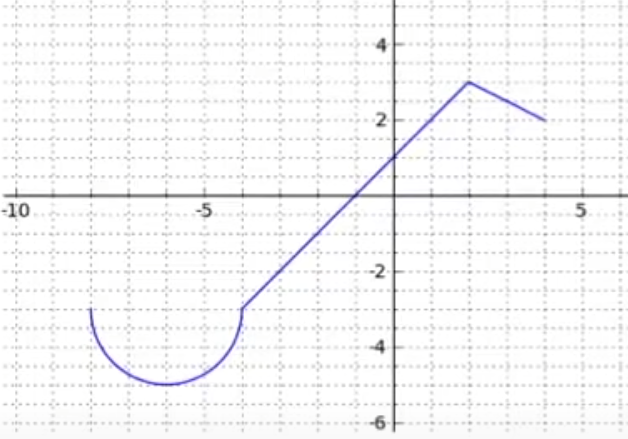
\includegraphics{algebra-pre-calculus/functions/graph1.png}
\end{align*}
\vspace{1pt}
What is $g(2)$ ? $ g(5) ?$ \\

First let's establish that $ y = g(x) $ so they are essentially mean the same thing. \\
In $g(2)$, $2$ corresponds to the $x$-value and we will use the graph to find corresponding $y$-value. \\
Since we know that we have to look for the $x$-value of $2$, we can look at the graph and find the point where $x = 2$. \\
Then we can look at the $y$-value of that point and that will be $3$. \\
Therefore, $g(2) = 3$. \\
Now when we look at $g(5)$, we can use the same method. However, we run into an issue that when we look at the x-value of $5$, we see that there is no point on the graph that has that x-value. \\
Therefore, $g(5)$ is undefined. \\
The question of what x-values and y-values makes sense to a function leads to the \textbf{domain} and \textbf{range} for a function. \\

\subsection{Domain and Range of a Function}
\textbf{Domain}: The domain of a function is the set of all possible x-values. \\
\textbf{Range}: The range of a function is the set of all possible y-values. \\

Let's examine the graph again and determine its range and domain. To find the domain of a function we have to look at the x-values that corresponds a point on the graph. \\
\begin{align*}
	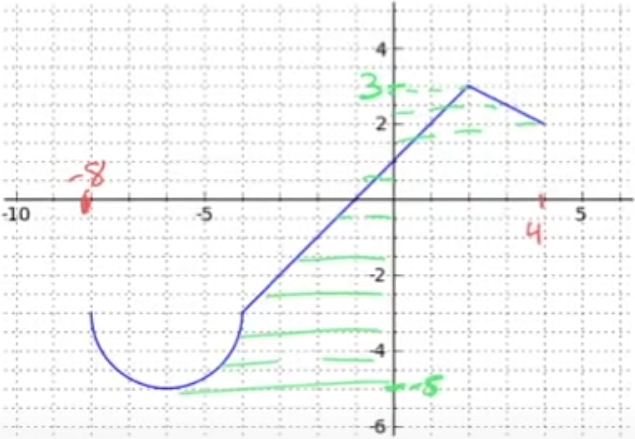
\includegraphics{algebra-pre-calculus/functions/graph2.png}
\end{align*}

We can see that the \textbf{domain} is $-8 \le x \le 4$. \\
Or as an interval notation, $[-8, 4]$. \\

To find the range of a function we have to look at the y-values that corresponds a point on the graph. \\
\textbf{range} is $-5 \le y \le 3$. \\
Or as an interval notation, $[-5, 3]$. \\

\subsection{Domain and Range of a Function as an Equation}
\textbf{Example}. Find the domain of these functions. \\
$\displaystyle A. \ g(x) = \frac{x}{x^2 - 4x + 3}$ \\
$\displaystyle B. \ f(x) = \sqrt{3-2x}$ \\
To find the domain of a function we have to consider algebraic restrictions. We can go ahead and question what values make sense to plug in for $x$. \\
Therefore,
\begin{itemize}
	\item 1. Exclude x-values that make the denominator 0.
	\item 2. Exclude x-values that make the radicand(number under the radical) negative. Since we cannot take the square root of a negative number.
\end{itemize}

What we have to do in the first function is this:
\begin{align*}
	x^2-4x+3 & \neq 0 \quad \text{Since the denominator cannot be 0} \\
\end{align*}

In other words we can solve the equation to be equal to 0 and exclude its solutions
\begin{align*}
	x^2-4x+3   & = 0 \quad \text{Factorise the quadratic} \\
	(x-3)(x-1) & = 0                                      \\
	x          & = 3, 1                                   \\
\end{align*}
Therefore we need to exclude $x=3$ and $x=1$ from the domain. \\

We can represent the domain as an interval notation. \\
\textbf{Domain} is $(-\infty, 1) \cup (1, 3) \cup (3, \infty)$. \\
Meaning that the domain is all real numbers except $1$ and $3$. \\

Now let's look at the second function.

Since we cannot take the square root of a negative number, we have to make sure that the radicand is not negative. \\

Therefore, we exclude the numbers:
$$ 3-2x < 0$$

Similarly we can include everyone number that makes the radicand positive(bigger than zero). \\
$$ 3-2x \ge 0$$
$$ 3 \ge 2x$$
$$ \frac{3}{2} \ge x$$

Therefore, the domain is $(-\infty, \frac{3}{2}]$.
Notice that we used a square bracket instead of a round bracket. This is because we can include the number $\frac{3}{2}$ in the domain. \\

\subsection{Function as a fractional equation with radicals}

\textbf{Example}. $\displaystyle h(x)=\frac{\sqrt{3-2x}}{x^2-4x+3}$ \\

So we have to consider the same restrictions as before. \\

\begin{align*}
	x^2-4x+3 &\neq 0 \quad \text{Since the denominator cannot be 0} \\
	3-2x &\ge 0 \quad \text{Since we cannot take the square root of a negative number} \\
\end{align*}

We've already solved the first condition which was $x\neq3$ and $x\neq1$. \\
The second condition is $x\le\frac{3}{2}$. \\

Therefore our domain is $(-\infty, 1) \cup (1, \frac{3}{2}]$.

\subsection{Increasing and Decreasing Functions}

\textbf{Example.} Which function is Increasing and which is Decreasing?

\begin{align*}
	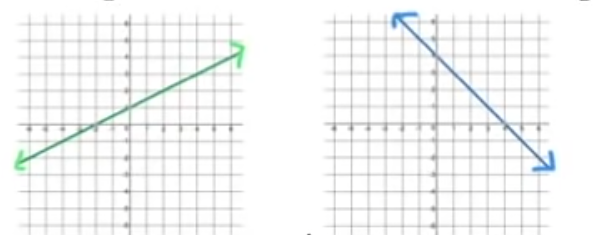
\includegraphics{algebra-pre-calculus/functions/graph3.png}
\end{align*}

As seen the first function is increasing and the second function is decreasing. 

This can be written more formaly as: \\
$ x_1 < x_2 \Rightarrow f(x_1) < f(x_2) $ \\
$x_1$ and $x_2$ are two arbitrary x-values. \\
This means that the y-values are increasing as the x-values are increasing. \\

In the decreasing function, the y-values are decreasing as the x-values are increasing. 
$ x_1 < x_2 \Rightarrow f(x_1) > f(x_2) $ \\

\textbf{Example.} On what intervals is the function graphed below increasing? Decreasing? 
\begin{align*}
	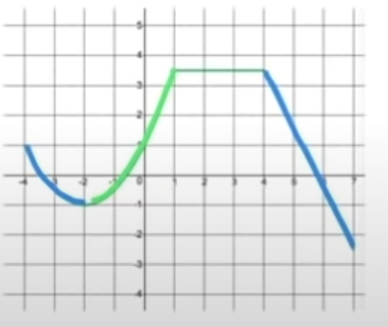
\includegraphics{algebra-pre-calculus/functions/graph4.png}
\end{align*}

We are going to solve this in terms of the x-values. Simply because the y-values can be same for different parts of the graph but the x-values are unique.
\textbf{Decreasing}: $-4\le x<-2, \quad 4<x\le7 $ \\
\textbf{Increasing}: $-2< x<1$ \\
As intervals: $[-4, -2) \cup (4,7), (-2, 1)$ \\

\subsection{Maximums and Minimums on Graphs}
\textbf{Definition.} An absolute maximum of a function, also known as a global maximum, is the highest value that the function can attain over its entire domain. In other words, it is the largest output (or y-value) that the function can produce for any input (or x-value) within its defined domain. \\
In other words a function f(x) has an absolute maximum at $x = c$ if $f(c) \ge f(x)$ for all $x$ in the domain of $f$. \\
The y-value f(c) is called the absolute maximum value of $f$. \\
and the point $(c, f(c))$ is called the absolute maximum point of $f$. \\

\begin{align*}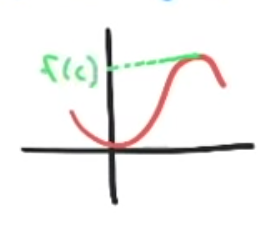
\includegraphics{algebra-pre-calculus/functions/graph5.png}\end{align*}
Here we can see that essentially the absolute maximum is the highest point on the graph. \\
And the absolute value point would be the point where it achieves the absolute maximum. \\
A function can have multiple absolute maximum points(multiple points referencing to the absolute maximum of the function), however it can only have one absolute maximum value. \\

\textbf{Definition}. The absolute minimum of a function, also known as a global minimum, is the lowest value that the function can attain over its entire domain. In other words, it is the smallest output (or y-value) that the function can produce for any input (or x-value) within its defined domain. \\
The absolute minimum of a function $f(x)$ is the smallest value of $f(x)$ over its entire domain. \\
In other words a function f(x) has an absolute minimum at $x = c$ if $f(c) \le f(x)$ for all $x$ in the domain of $f$. \\
The y-value f(c) is called the absolute minimum value of $f$. \\
and the point $(c, f(c))$ is called the absolute minimum point of $f$. \\

\begin{align*}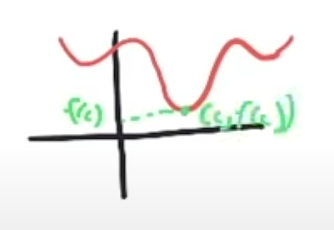
\includegraphics{algebra-pre-calculus/functions/graph6.png}\end{align*}
Here we can see that essentially the absolute minimum is the lowest point on the graph. \\
And the absolute value point would be the point where it achieves the absolute minimum. \\
A function can have multiple absolute minimum points(multiple points referencing to the absolute minimum of the function), however it can only have one absolute minimum value. \\
\newpage
\subsection{Local Maximums and Minimums}
\textbf{Definition.} A local maximum of a function is a point on the graph where the y-value is greater than or equal to all the y-values of points in the nearby region. \\
A function f(x) has a local maximum at $x = c$ if $f(c) \ge f(x)$ for all $x$ in some open interval around $c$. \\

In other words, the way we identify local maximums is by looking at the graph and seeing if there is a point where an interval around that point exists such that all function values within that interval are less than or equal to the function value at that specific point. If this condition is met, we can conclude that the function has a local maximum at that point.

A local minimum of a function is a point on the graph where the y-value is less than or equal to all the y-values of points in the nearby region. \\
A function f(x) has a local minimum at $x = c$ if $f(c) \le f(x)$ for all $x$ in some open interval around $c$. \\
In other words, the way we identify local minimums is by looking at the graph and seeing if there is a point where an interval around that point exists such that all function values within that interval are greater than or equal to the function value at that specific point. If this condition is met, we can conclude that the function has a local minimum at that point. \\

\textbf{Definition}. Local maximum and minimum points are also called relative maximum and minimum points. \\
\textbf{Definition}. A point where a function changes from increasing to decreasing or decreasing to increasing is called a turning point. \\

\newpage
\begin{figure}
	\centering
	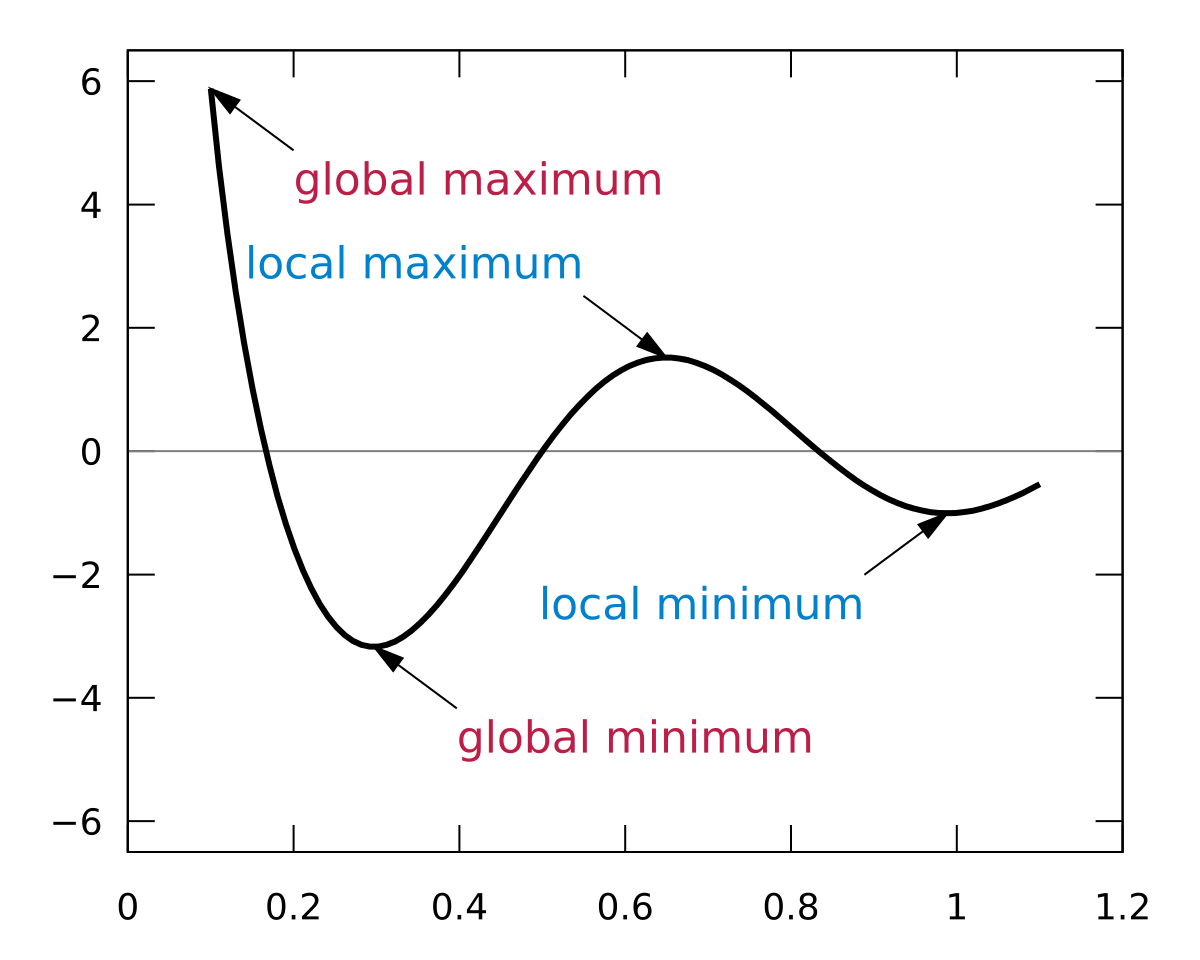
\includegraphics[width=0.5\textwidth]{algebra-pre-calculus/functions/graph7.png}
	\caption{Absolute Maximum and Minimum with Local Maximum and Minimum}
\end{figure}

\subsection{Example}


\begin{align*}
	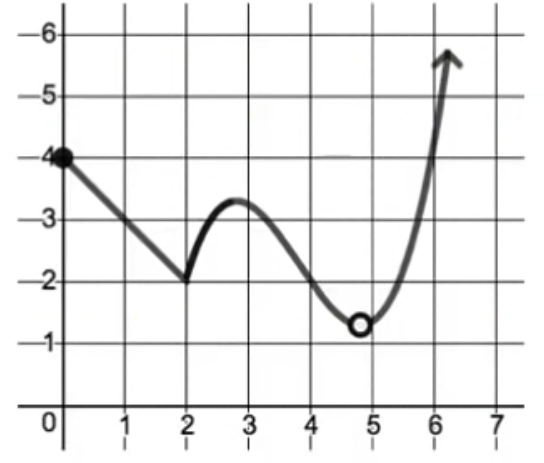
\includegraphics{algebra-pre-calculus/functions/example_graph.png}
\end{align*}

\textbf{Example.} 
\begin{enumerate}
	\item Mark all local maximum and minimum points on the graph. 
	\item Mark all absolute maximum and minimum points on the graph.
	\item What are the local maximum and minimum values?
	\item What are the absolute maximum and minimum values?
\end{enumerate}

\textbf{Solution.} \\
The function has a local maximum point here: $(2.7,-3.3)$ \\
There is a local minimum point here: $(2, 2)$ \\
The point with the drilled out circle means that it is not part of the graph. If it would be then that point would be a local minimum point and an absolute minimum point. \\ 
The point $(0,4)$ by some sources considered to be a local maximum point, However by other sources it doesn't. 
Therefore, we do not have any absolute maximum points, as the arrow indicates that the function goes to infinity. \\
We don't have any absolute minimum points either. \\
Now for talking about the values, we can see that the local maximum value is $-3.3$ and the local minimum value is $2$ which are just the y-values of the points. \\
We do not have any absolute maximum or minimum values.
 % Section 7 - Functions
% Chapter 1 end - Algebra

% % Chapter 2 - Linear Algebra
% \chapter{Linear Algebra}
% The second chapter is about linear algebra. It will cover the topics that was written by Gábor Hadházy and Tamás Hadházy.
% \section{Linear Equations}

A linear equation is an equation in which the highest power of the variable is always 1. It is also known as a one-degree equation. 
Additionally A linear equation is an equation that can be written as the sum of numbers(coefficients) times variables, added up to equal to a number.

For example. $ 2x + 3y + 7.3z = 5 $ is a linear equation.

\begin{itemize}
    \item $4x^2 + 5x + 6 = 0$ is not a linear equation because the highest power of the variables is 2.
    \item $ \frac{1}{3}uv + \frac{2}{3}u = \frac{3}{5}v $ is not a linear equation because it includes a product of variables.
    \item $ 5a + 2 = 6b - \sqrt[]{2c}  $ is a linear equation because if we rearrange it, we will get: 
    $$ 5a - 6b + \sqrt[]{2c} = -2 $$
\end{itemize}

a system of linear equations (or linear system) is a collection(set) of one or more linear equations involving the same variables

For example, 
\begin{align*}
    3x + 2y - z &= 1 \\
    2x - 2y + 4z &= -2 \\
    -x + \frac{1}{2}y -z &= 0
\end{align*}
is a system of three equations in the three variables $x, y, z$. A solution to a linear system is an assignment of values to the variables such that all the equations are simultaneously satisfied. \\
A solution to the system above is given by the ordered tuple.
$$ {\displaystyle (x,y,z)=(1,-2,-2)} $$  
\subsection{Solving systems of Linear Equations with the method of substitution}
It is important to establish that there are limitless ways to solve systems of linear equations. 
Example. Solve the system of linear equations(we are going to use the method of substitution): 
\begin{align*}
    -2a + 3b + 4c = 1 \\
    a + b + 5c = 2 \\
    b = 2a + c
\end{align*}
Firstly we already have a value for $b$ in the 3rd equation so let's just substitute it into the first two equations.
\begin{align*}
    &1. \quad -2a + 3(2a + c) + 4c = 1 \\
    &2. \quad a + (2a + c) + 5c = 2 \\ 
    &3. \quad  b = 2a + c   
\end{align*}

Let's simplify the first two equations.
After expanding and simplifying the first two terms we will get:
\begin{align*}
    &1.\quad 4a + 7c = 1 \\
    &2.\quad 3a + 6c = 2 \\
    &3.\quad b = 2a + c      
\end{align*}
Notice that now we have two equations with two variables, so we can solve for $a$ and $c$.
\\ 

\begin{itemize}
    \item In the first equation we can subtract $7c$ and then divide by $4$ to get $a$. Which will give us: 
    \begin{align*}
        1. \quad  a = \frac{1}{4} - \frac{7}{4}c \\
        2. \quad 3a + 6c = 2 \\
        3. \quad b = 2a + c
    \end{align*}
    \item Now that we have the value for $a$ we can substitute that into the second equation. Which will give us:
    \begin{align*}
        &1. \quad a = \frac{1}{4} - \frac{7}{4}c \\
        &2. \quad 3(\frac{1}{4} - \frac{7}{4}c) + 6c = 2 \\
        &3. \quad b = 2a + c
    \end{align*}
    \item Now let's simplify the second equation. After expanding and simplifying with the like terms we will get:
    \begin{align*}
        &1. \quad a = \frac{1}{4} - \frac{7}{4}c \\
        &2. \quad \frac{3}{4} - \frac{21}{4}c + 6c = 2 \xrightarrow{\text{add like terms}} \frac{3}{4} + \frac{3}{4}c = 2\\
        &3. \quad b = 2a + c
    \end{align*}
    \item Now that we have this, we can simply subtract $\frac{3}{4}$ then simplify it down to: 
    $$ c = \frac{5}{3} $$ 
    \item Since we have the value for $c$ now let's figure out the value for $a$.
    $$ a = \frac{1}{4} - \frac{7}{4}(\frac{5}{3}) = \frac{1}{4} - \frac{35}{12} = - \frac{32}{12} = -\frac{8}{3}$$
    Therefore, $ a = - \frac{8}{3} $
    \item Now that we have the value for $a$ and $c$ we can substitute that into the third equation to get the \textbf{actual} value for $b$.
    $$ b = 2(-\frac{8}{3}) + \frac{5}{3} = -\frac{16}{3} + \frac{5}{3} = -\frac{11}{3}$$
\end{itemize}

Now finally we have solved the system of linear equations and we have the values for $a, b, c$. If we'd plug them in into the original equations then it would satisfy all of them. \\ 
We can list the values in an ordered tuple like this:
$$ {\displaystyle (a,b,c)=(-\frac{8}{3},-\frac{11}{3},\frac{5}{3})} $$
Now let's see another way of solving systems of linear equations.
\subsection{Solving systems of Linear Equations with the method of elimination}
Example. Solve the system of linear equations(we are going to use the method of elimination): 
\begin{align*}
    &1. \quad -2a + 3b + 4c = 1 \\
    &2. \quad a + b + 5c = 2 \\ 
    &3. \quad  b = 2a + c   
\end{align*}
Let's rearrange this system by writing each equation in the standard form, where all the variables are on the left side and the constants are on the right side.
The first two equations are already in the standard form, but the third one is not. So let's rearrange it.

\begin{align*}
    &1. \quad -2a + 3b + 4c = 1 \\
    &2. \quad a + b + 5c = 2 \\ 
    &3. \quad  -2a + b - c = 0  
\end{align*} % Section 1 - Linear Equations


\end{document}